\newpage

\section{Map Editor}
This section describes how you can edit existing maps or create new maps from scratch. This can be done with a editing tool, or by directly editing the map files manually.




\subsection{Using the Environment Store}
The Map Editor is a tool for editing maps for the BW4T server. Double click the jar file environment-store.jar  in the $<$SERVER$>$ directory to start the  editor.

\begin{wrapfigure}{r}{0.4\textwidth}
  \begin{center}
    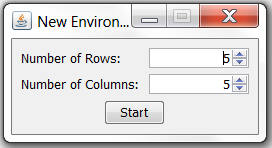
\includegraphics[width=0.4\textwidth]{EnvironmentStore/SizeDialog.png}
  \end{center}
  \caption{Choose the amount of columns and rows}\label{fig:MapSize}
\end{wrapfigure}


After starting up, the map size dialog (Figure \ref{fig:MapSize}) appears, which can be used as follows.
Here you can choose the amount of rows and columns you want the environment to consist of. Each cell in the "table" can be used to fulfill one piece of the map. This could either be a room, a corridor, a dropzone, a charging zone, start zone or a blockade. By pressing the colours at the bottom you can generate the sequence to be completed. This can also be done by pressing the according numbers on the keyboard. 



At the moment, for an existing map to be loaded in the map editor, the correct sizes of the map have to be entered before the map can be loaded.

% we put the figure early, to allow tex to be more flexible with
% the placement. Even this may be insufficient....
\begin{figure}
	\center
	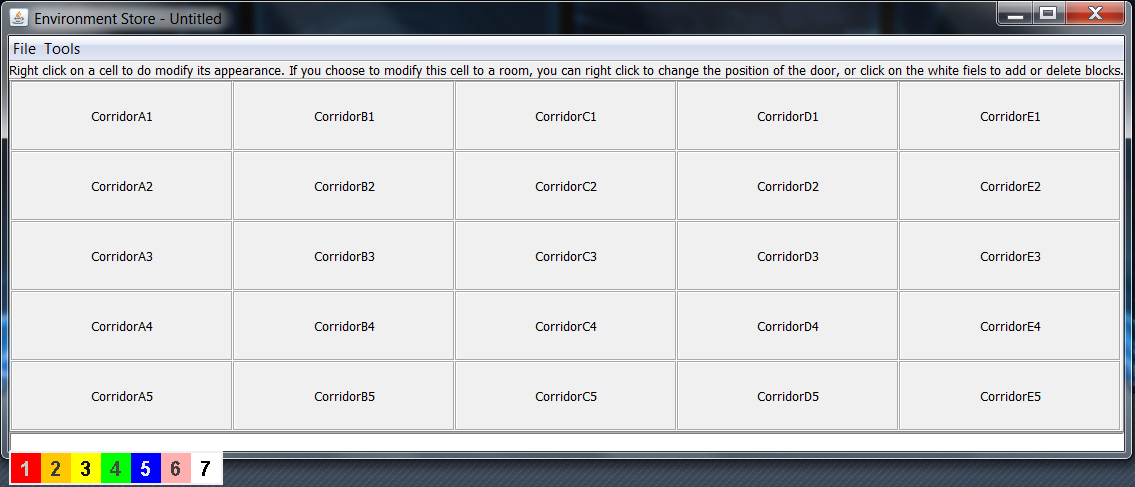
\includegraphics[scale=0.55]{EnvironmentStore/MapEditor.png}
	\caption{the map editor with a 5x5 freshly created map}\label{fig:MapEditor}
\end{figure}

In the Map editor GUI above you can add blocks to rooms. To add blocks to rooms, right click in the cell, adjust the type of the zone to Room. Now you can add blocks the way you did with the sequence. Right clicking the cell again lets you choose at which side of the room you want the door. When you're done, press save. 
By pressing Tools in the menu bar, you are able to randomize zones, blocks and sequences.

WARNING: Randomizing these will not always guarantee that the sequence can be completed. By pressing File in the menu bar, you are able to watch a preview of your map, and you are able to save the map. Save the map in the $<$SERVER$>/$maps folder \footnote[1]{This map directory appears after the first run of the server.}.  


\begin{wrapfigure}{r}{0.3\textwidth}
  \begin{center}
		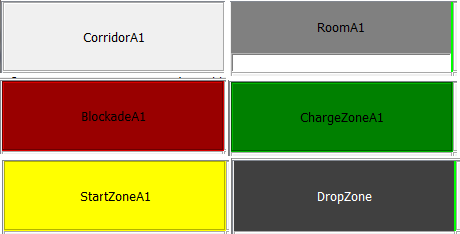
\includegraphics[width=0.3\textwidth]{EnvironmentStore/DifferentRooms.png}
  \end{center}
\caption{the color palette at the bottom of the map editor}\label{fig:DifferentRooms}

\end{wrapfigure}

\subsection{Map editor}
After specifying the amount of rows and columns the map should have, and clicking on the Start button, 
the map editor is launched. Figure \ref{fig:MapEditor} shows the environment store after launch, with a 5x5 map.

The map editor has many functionalities. The functionalities are detailed bit by bit in this documentation.


\subsection{Editing a room}

Right click on any corridor (or any zone of the matrix for that matter), and the drop down menu is shown (Figure \ref{fig:DropDownMenuRoom}).

This allows a zone to be converted to any one of a corridor, a room, a blockade, a charge zone, a start zone, and a drop zone. Figure \ref{fig:DifferentRooms} shows the different appearances of the zones in the map editor.

 \begin{figure}
        \centering
        \begin{subfigure}[b]{0.48\textwidth} % 0.5 may give 2 rows instead of 2 colums
        	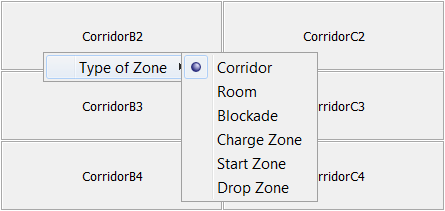
\includegraphics[width=0.8\textwidth]{EnvironmentStore/DropDownMenuRoom.png}
	\caption{the drop down menu generated when a zone is right clicked}\label{fig:DropDownMenuRoom}
        \end{subfigure}
        \begin{subfigure}[b]{0.48\textwidth}
	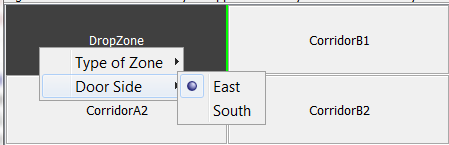
\includegraphics[width=0.8\textwidth]{EnvironmentStore/DropDownMenuRoom2.png}
	\caption{the drop down menu generated when a room is right clicked}\label{DropDownMenuRoom2}
        \end{subfigure}
        \caption{Drop Down menus}\label{fig:animals}
\end{figure}

As can be seen, the room and drop zone contain a green border. This is to indicate which way the door to enter the room is faced. This is also editable. When right clicking on a certain room, a drop down menu pops up (Figure \ref{DropDownMenuRoom2}). This drop down menu lists the directions the door can face while still being accessible. In this case, as it is the top left zone, only doors facing east or south are possible.




\subsection{Editing a sequence}
Under the zones of the map editor is a white rectangle that contains the sequence for that map. This same rectangle is also present in the rooms that aren't drop zones (Figure \ref{fig:SequenceEditor}).

\begin{figure}
	\center
	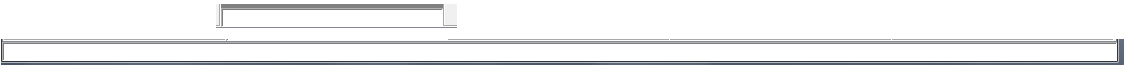
\includegraphics[scale=0.5]{EnvironmentStore/SequenceEditor.png}\\
	\caption{The rectangle at the bottom of both the map editor and the rooms.}\label{fig:SequenceEditor}
\end{figure}

The rectangle in the rooms can be used to enter colors, which are then used in the blocks that are placed in that room. The rectangle under the zones can be used to enter the colors that make up the sequence that has to be completed for that map. To add colors, the color palette is useful.
\subsection{Color palette}
At the bottom of the map editor is the color palette. A larger picture is given in Figure \ref{fig:ColorPalette}.

\begin{figure}[h!]
	\center
	
\includegraphics{EnvironmentStore/ColorPalette.png}
	\caption{the color palette at the bottom of the map editor.}
	\label{fig:ColorPalette}
\end{figure}



The color palette is used for adding blocks to rooms and the sequence to be completed in the map. When clicking on the box containing either the sequence of the map or the blocks in the room, the color palette is shown. It allows for the adding of colors by clicking on the respective colors on the palette, but colors can also be added by entering the respective numbers in the colors (pressing 1 adds a red block to the room or sequence, for example) and also by entering the first letter of the color (so pressing R adds a red block).

 \begin{figure}[h!]
        \centering
        \begin{subfigure}[b]{0.48\textwidth} % 0.5 may give 2 rows instead of 2 colums
	\center
	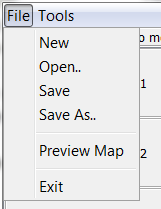
\includegraphics{EnvironmentStore/DropDownFile.png}
	\caption{the drop down menu created when the 'File' menu item is clicked.}
	\label{fig:DropDownFile}
        \end{subfigure}
        \begin{subfigure}[b]{0.48\textwidth}
	\center
	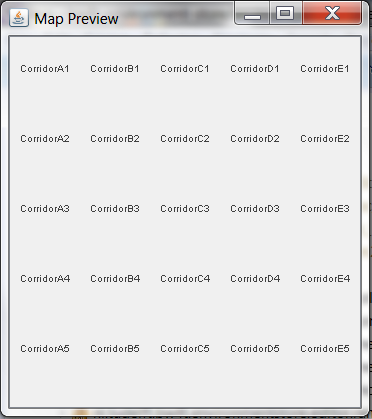
\includegraphics[width=0.9\textwidth]{EnvironmentStore/Preview.png}
	\caption{The preview of a 5x5 non-edited map, with no blocks in the sequence.}
	\label{fig:Preview}
        \end{subfigure}
        \caption{Drop Down menus}
\end{figure}

\subsection{File menu}
The file menu (Figure \ref{fig:DropDownFile}) contains not only the standard operations for exporting a created map to a file, so that it can be used later, but also a few other options.

The New-, Open...-, Save- and Save as...-options are the standard file operations and need no further explanation. However, as added functionality to the options, it is impossible to save a map not containing either a start- or drop zone, as well as a map not containing a block in its sequence, and saving an unsolvable map will give a warning describing what's wrong. The Exit-option also needs no further explanation. The Preview-option gives a preview of the created map, as how it would be rendered when used as an actual map for bots. For a non-edited 5x5 map, the preview looks as shown in Figure \ref{fig:Preview}.

 \begin{figure}[h!!!]
        \centering
        \begin{subfigure}[b]{0.32\textwidth} 
	\center
	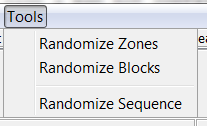
\includegraphics[width=0.9\textwidth]{EnvironmentStore/DropDownTools.png}
	\caption{The drop down menu created when the 'Tools' menu item is clicked.}
	\label{fig:DropDownTools}
        \end{subfigure}
        \begin{subfigure}[b]{0.32\textwidth}
	\center
	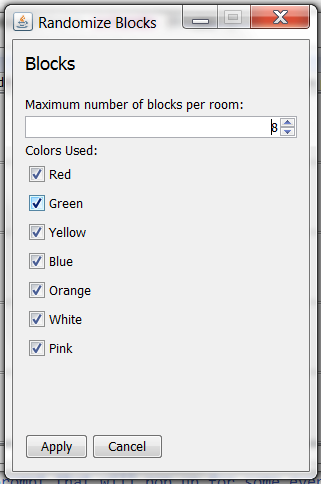
\includegraphics[width=0.9\textwidth]{EnvironmentStore/MenuBlocks.png}
	\caption{The menu appearing when the randomize blocks option is clicked in the menu.}
	\label{fig:MenuBlocks}
        \end{subfigure}
        \begin{subfigure}[b]{0.32\textwidth}
	\center
	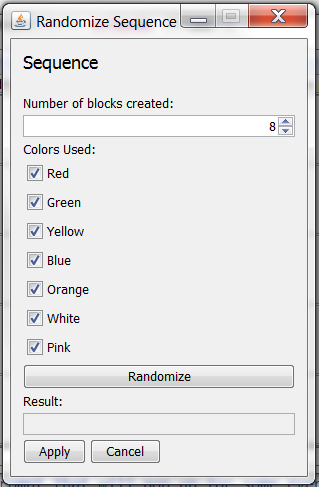
\includegraphics[width=0.9\textwidth]{EnvironmentStore/MenuSeq.png}
	\caption{The menu appearing when the randomize blocks option is clicked in the menu.}
	\label{fig:MenuSeq}
        \end{subfigure}

        \caption{menus}\label{fig:whatever}
\end{figure}

\subsection{Tools menu}
The other drop down menu at the top of the map editor is the tools menu (Figure \ref{fig:DropDownTools}). This menu contains options to use several tools.

Clicking on the 'Randomize Zones' option creates a random map, based off a vanilla map with reclassification of rooms to blockades, charge zones or corridors, and with reclassifications of existing corridors to charge zones. The map is always solvable, given that all the blocks in the sequence are present in the map and no further changes are made to the map. The 'Randomize Blocks' option randomizes the blocks contained in every room according to parameters that the user has to specify. Figure 	\ref{fig:MenuBlocks} shows the menu.

This interface allows the user to specify which block colors they want to be spawned, and also the max. amount of blocks in a room. The interface for random sequence generation is slightly different (Figure \ref{fig:MenuSeq}).



The differences between this interface and the previous interface are the Randomize button and Result label, that  create and display resp. the random sequence, and the apply and cancel button which enter the sequence in the map or cancel the creation of the sequence, respectively.


\subsection{Manual editing of Maps}
It is also possible to manually edit a map as it is a plain text XML file.
\begin{enumerate}
\item Copy an existing map file in the $<$SERVER$>/$maps folder to a new file \footnotemark[1].
\item Open the copied map with a text editor. You can then edit the colors in the rooms. Each $<$blocks$>$COL$</$blocks$>$ line inside a $<$zones$>$ of type ROOM adds another block to the room. The currently available colors are BLUE, ORANGE, RED, WHITE, GREEN, YELLOW AND PINK. A room has place for at most 10 blocks.
\item You can change the number of rooms by adding or removing $<$zones$>$ of type ROOM and position the rooms correctly on the map by editing the $<$x$>$ $<$y$>$ $<$width$>$ and $<$height$>$ inside the room's $<$boundingbox$>$. Also you need to add a $<$door$>$ properly positioned on the border of the room.
\item You can edit the goal sequence by adding $<$sequence$>$ items to the map, with colors as mentioned above.
\item You can prevent multiple entities to enter corridor zones by putting true in the item $<$oneBotPerCorridorZone$>$ in the map.
\item You can add entities to the environment by creating more $<$entities$>$ items. Make sure they have a unique $<$name$>$ and that their start position is in a different $<$zone$>$ if you have $<$oneBotPerCoridorZoneidorZone$>$ set to true.
\item You can let the server pick a random sequence of a given length by setting the $<$randomSequence$>$ to a positive value. These random blocks are added to the existing sequence items and the random blocks are placed randomly on the map.
\item You can let the server pick random extra blocks to be placed in the rooms on the map by putting a positive number in the $<$randomBlocks$>$ in the map. Note that this addition is on top of all blocks that are already placed in the map; so normally you leave the room zones empty when using this option.
\item You can set per-zone visibility of the zone namelabel in the server map renderer, using a $<$renderOptions$>$ $<$labelVisible$>$ false $</$labelVisible$>$ $</$renderOptions$>$ block to disable visibility.
\item Save the map in the $<$SERVER$>/$maps directory.
\item Edit the map initialization parameter for the server to your new map file. See the section on customizing the server settings. If you now start the server and your new map should be loaded.
\end{enumerate}


